\chapter{Diagrammes d'Ellingham et métallurgie}\label{ch:b2:ellingham}

Un haut fourneau transforme une roche rouge en fonte liquide avec du coke et de l'air chaud,
au rythme de milliers de tonnes par jour. Aucun four de ce type ne produira jamais
d'aluminium, de magnésium ou de titane, bien que le carbone soit tout aussi bon marché pour eux.
La plupart des métaux se trouvent dans le sol sous forme d'oxydes, et obtenir un métal, c'est
lui retirer son oxygène~: quels réducteurs le peuvent, et à quelle
température, c'est une question d'\omterm{def:b2:reaction-free-energy:gibbs-energy}{enthalpies libres} standard. En 1944, Harold
Ellingham les a toutes tracées sur un même graphique, en fonction de la température, pour une mole de
dioxygène chacune. Ce diagramme indique d'un coup d'œil quel métal réduit quel oxyde,
pourquoi le carbone l'emporte à haute température, et pourquoi certains métaux doivent être produits par
électrolyse.

\begin{recall}
\Cref{ch:b2:reaction-free-energy}~: $\Delta_r G^\circ = \Delta_r H^\circ -
T\Delta_r S^\circ$ et l'\omterm{def:b2:reaction-free-energy:ellingham-approximation}{approximation d'Ellingham} (droites en $T$,
changements d'état exceptés). \Cref{ch:b2:equilibrium-shifts}~: $K^\circ$ à partir de
$\Delta_r G^\circ$, \omterm{def:b2:equilibrium-shifts:variance}{variance}, fin d'un équilibre par disparition d'une
phase. Le volume de première année~: nombres d'oxydation, couples oxydant-réducteur, oxydes basiques et
acides. Le volume scolaire~: les minerais.
\end{recall}

\begin{omfigure}
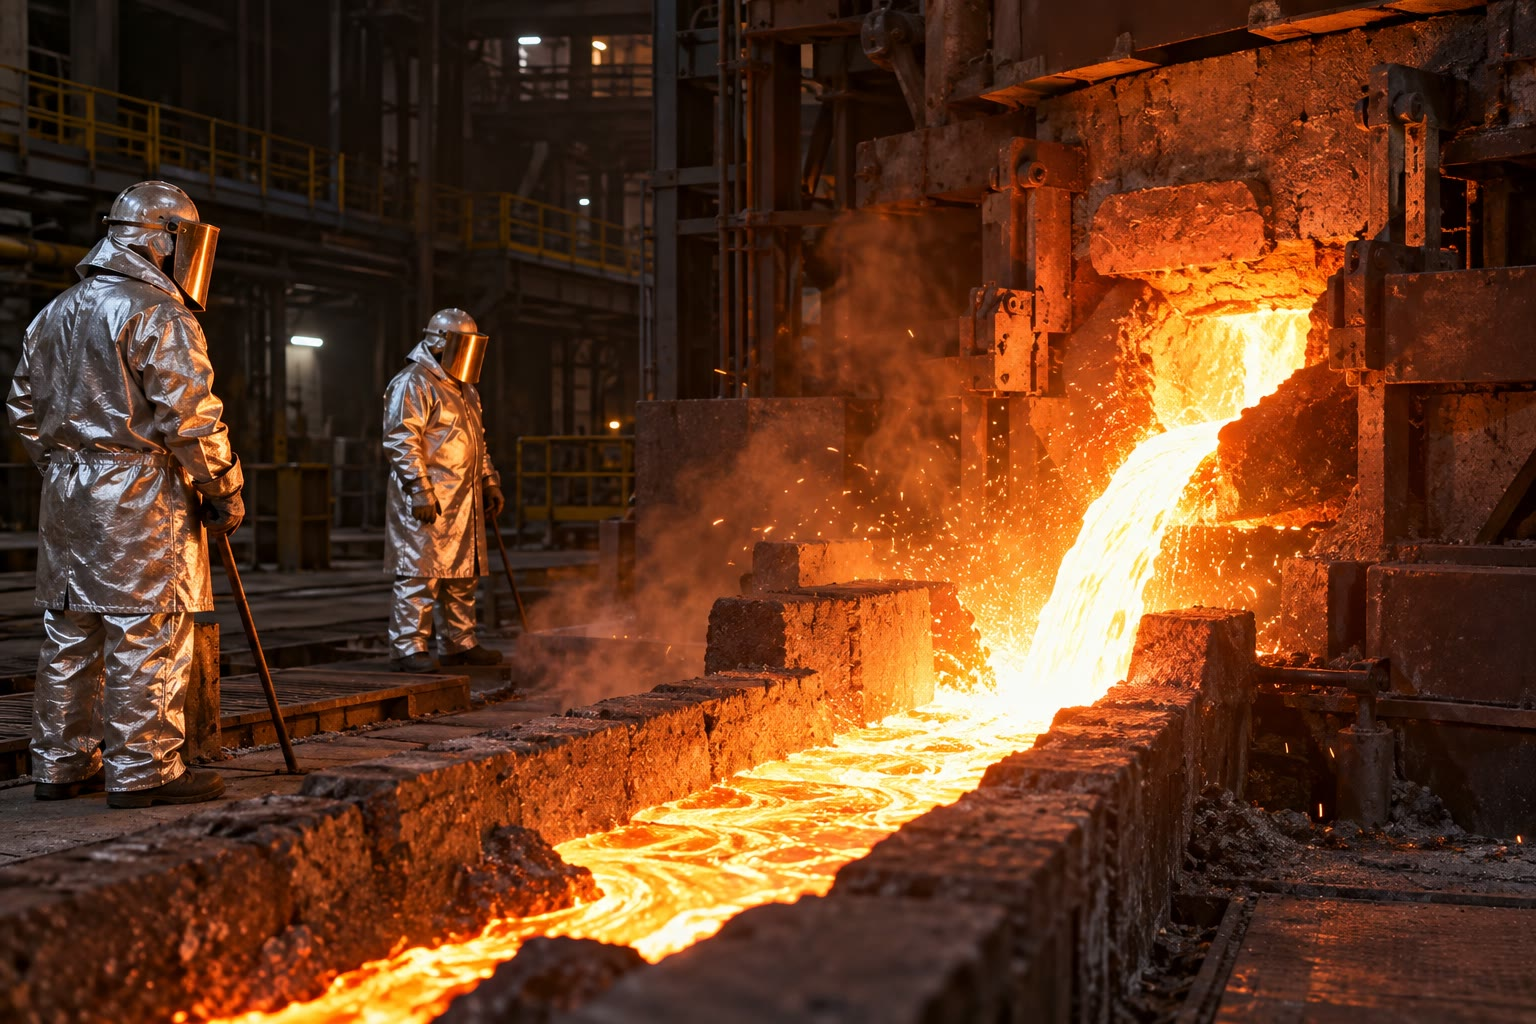
\includegraphics[width=0.62\linewidth]{images/book3/ai/b2-06-blast-furnace.jpg}

{\small Coulée d'un haut fourneau~: la fonte liquide s'écoule dans une rigole réfractaire,
sous l'œil d'ouvriers en combinaison réfléchissante. La température et le gaz
à l'intérieur du four sont ceux qui permettent au monoxyde de carbone d'arracher l'oxygène
de l'oxyde de fer.}
\end{omfigure}

\section{Le diagramme d'Ellingham}

Pour comparer l'affinité de différents métaux pour l'oxygène, on écrit les réactions
de sorte qu'elles consomment toutes la même quantité du réactif commun.

\begin{definition}[Diagramme d'Ellingham]\label{def:b2:ellingham:diagram}
Le \emph{diagramme d'Ellingham}\index{diagramme d'Ellingham} d'une famille d'oxydes
est la représentation, en fonction de la température, des \omterm{def:b2:reaction-free-energy:gibbs-energy}{enthalpies libres} standard de leurs
réactions de formation écrites pour une mole de dioxygène,
\[
  \tfrac{2x}{y}\,\mathrm M + \ce{O2} \longrightarrow \tfrac{2}{y}\,\mathrm{M}_x\mathrm O_y ,
  \qquad \Delta_r G^\circ(T) \ \text{par mole de } \ce{O2} .
\]
\end{definition}

Par exemple \ce{2Zn + O2 -> 2ZnO}, \ce{4/3Al + O2 -> 2/3Al2O3}, \ce{2C + O2 ->
2CO}. L'ordonnée est en \unit{kJ} par mole de \ce{O2}, toujours négative pour les
métaux du diagramme.

\begin{proposition}[Des droites]\label{prop:b2:ellingham:line}
Dans l'\omterm{def:b2:reaction-free-energy:ellingham-approximation}{approximation d'Ellingham}, chaque tracé est une droite de pente $-\Delta_r
S^\circ$. Pour un métal et son oxyde, tous deux condensés, $\Delta_r S^\circ$ est
proche de l'opposé de l'entropie de la mole de dioxygène consommée, soit environ
$-\qty{200}{J/(K.mol)}$~: les droites montent avec la température, toutes avec presque la
même pente.
\end{proposition}

\begin{proof}
$\Delta_r G^\circ = \Delta_r H^\circ - T\Delta_r S^\circ$ avec $\Delta_r
H^\circ$, $\Delta_r S^\circ$ constantes. Les entropies molaires des solides valent quelques dizaines de
\unit{J/(K.mol)} et se compensent largement entre métal et oxyde, tandis qu'une mole de
gaz est consommée, d'entropie $S^\circ(\ce{O2}) = \qty{205}{J/(K.mol)}$. Pour le zinc,
$2(43.65) - 2(41.63) - 205.15 = \qty{-201.1}{J/(K.mol)}$.
% ledger: s0:ZnO_cr, s0:Zn_cr, s0:O2_g
\end{proof}

\begin{proposition}[Ruptures de pente]\label{prop:b2:ellingham:break}
À la température où le métal fond ou bout, la droite change de pente~:
sa pente augmente de $\nu\,\Delta_{\text{trs}}S$, où $\nu$ est la quantité de
métal dans la réaction et $\Delta_{\text{trs}}S = \Delta_{\text{trs}}H/T_{\text{trs}}$.
Un changement d'état de l'oxyde diminue au contraire la pente.
\end{proposition}

\begin{proof}
Au-dessus du changement d'état, le métal réagit à partir de sa nouvelle phase, dont l'entropie est
plus grande de $\Delta_{\text{trs}}S$~: $\Delta_r S^\circ$ diminue de $\nu\,\Delta_{\text{trs}}S$
et la pente $-\Delta_r S^\circ$ augmente d'autant. $\Delta_r G^\circ$
elle-même est continue, car en $T_{\text{trs}}$ les deux phases ont le même
\omterm{def:b2:chemical-potential:chemical-potential}{potentiel chimique}. Pour l'oxyde, le signe est opposé.
\end{proof}

La fusion change un peu la pente~; l'ébullition, qui transforme un réactif condensé
en gaz, la change beaucoup. Le zinc bout à \qty{1180}{K}~: au-dessus de cette
température, la formation de l'oxyde de zinc consomme trois moles de gaz pour deux d'oxyde,
et sa droite monte fortement. Il en va de même pour le magnésium au-dessus de sa
température d'ébullition.

\begin{omfigure}
\begin{tikzpicture}[lab/.style={anchor=west, font=\scriptsize, inner sep=1pt}]
\begin{axis}[omellingham,
  width=0.84\linewidth, height=11cm, xmin=300, xmax=2100, ymin=-1250, ymax=0,
  clip mode=individual,
  xlabel={$T$ (K)}, ylabel={$\Delta_r G^\circ$ (\unit{kJ} par mol de \ce{O2})},
  xtick={300,500,700,900,1100,1300,1500,1700,1900,2100},
  x tick label style={rotate=45, anchor=north east, font=\scriptsize}]
\addplot[black!60, thick] table[x=T, y=G] {figdata/out/bachelor-2-ellingham-a-HgO.dat};
\addplot[omProp, thick] table[x=T, y=G] {figdata/out/bachelor-2-ellingham-a-Cu2O.dat};
\addplot[omDef, thick] table[x=T, y=G] {figdata/out/bachelor-2-ellingham-a-FeO.dat};
\addplot[omExo, very thick] table[x=T, y=G] {figdata/out/bachelor-2-ellingham-a-ZnO.dat};
\addplot[black!60, thick] table[x=T, y=G] {figdata/out/bachelor-2-ellingham-a-Cr2O3.dat};
\addplot[omProp, thick] table[x=T, y=G] {figdata/out/bachelor-2-ellingham-a-TiO2.dat};
\addplot[omDef, thick] table[x=T, y=G] {figdata/out/bachelor-2-ellingham-a-Al2O3.dat};
\addplot[black!60, thick] table[x=T, y=G] {figdata/out/bachelor-2-ellingham-a-MgO.dat};
\addplot[omProp, thick] table[x=T, y=G] {figdata/out/bachelor-2-ellingham-a-CaO.dat};
\addplot[omThm, very thick] table[x=T, y=G] {figdata/out/bachelor-2-ellingham-a-C-CO.dat};
\addplot[omThm, thick, dashed] table[x=T, y=G] {figdata/out/bachelor-2-ellingham-a-C-CO2.dat};
\addplot[omThm, thick, dotted] table[x=T, y=G] {figdata/out/bachelor-2-ellingham-a-CO-CO2.dat};
\addplot[omDef, thick, dashed] table[x=T, y=G] {figdata/out/bachelor-2-ellingham-a-H2-H2O.dat};
% labels: inside for the two short lines, at the right end for the others
\node[font=\scriptsize, black!70, anchor=south] at (axis cs:400,-60) {\ce{HgO}};
\node[font=\scriptsize, omProp, anchor=south] at (axis cs:1100,-150) {\ce{Cu2O}};
\draw[omExo, thin] (axis cs:2100,-69) -- (axis cs:2150,-60) node[lab, text=omExo] {\ce{ZnO}};
\draw[omThm, thin] (axis cs:2100,-204) -- (axis cs:2150,-185) node[lab, text=omThm] {\ce{CO}/\ce{CO2}};
\draw[omDef, thin] (axis cs:2100,-259) -- (axis cs:2150,-235) node[lab, text=omDef] {\ce{H2}/\ce{H2O}};
\draw[omDef, thin] (axis cs:2100,-286) -- (axis cs:2150,-285) node[lab, text=omDef] {\ce{FeO}};
\draw[black!70, thin] (axis cs:2100,-393) -- (axis cs:2150,-365) node[lab, text=black!70] {\ce{Cr2O3}};
\draw[omThm, thin] (axis cs:2100,-396) -- (axis cs:2150,-415) node[lab, text=omThm] {\ce{C}/\ce{CO2}};
\draw[omProp, thin] (axis cs:2100,-567) -- (axis cs:2150,-540) node[lab, text=omProp] {\ce{TiO2}};
\draw[omThm, thin] (axis cs:2100,-589) -- (axis cs:2150,-590) node[lab, text=omThm] {\ce{C}/\ce{CO}};
\draw[black!70, thin] (axis cs:2100,-600) -- (axis cs:2150,-640) node[lab, text=black!70] {\ce{MgO}};
\draw[omDef, thin] (axis cs:2100,-668) -- (axis cs:2150,-690) node[lab, text=omDef] {\ce{Al2O3}};
\draw[omProp, thin] (axis cs:2100,-765) -- (axis cs:2150,-765) node[lab, text=omProp] {\ce{CaO}};
\end{axis}
\end{tikzpicture}

{\small Le \omterm{def:b2:ellingham:diagram}{diagramme d'Ellingham}~: \omterm{def:b2:reaction-free-energy:gibbs-energy}{enthalpie libre} standard de formation des oxydes
par mole de \ce{O2}, en fonction de la température, d'après les \omterm{def:b2:reaction-free-energy:gibbs-energy}{enthalpies libres} tabulées. Plus
une droite est basse, plus l'oxyde est stable et plus le métal est réducteur.
Chaque droite de métal porte le nom de son oxyde~; \ce{C}/\ce{CO} désigne \ce{2C + O2 -> 2CO},
\ce{C}/\ce{CO2} désigne \ce{C + O2 -> CO2}, \ce{CO}/\ce{CO2} désigne \ce{2CO + O2 -> 2CO2}
et \ce{H2}/\ce{H2O} désigne \ce{2H2 + O2 -> 2H2O}, l'eau étant gazeuse.}
% ledger: janafG:Cu2O.300, janafG:FeO.300, janafG:Cr2O3.300, janafG:TiO2.500, janafG:Al2O3.300, janafG:MgO.300, janafG:CaO.300, janafG:CO.300, janafG:CO2.300, janafG:H2O.300, dfh:ZnO_cr, dfh:HgO_cr, s0:HgO_cr, s0:Hg_l, s0:Hg_g, dfh:Hg_g (all temperatures in figdata/bachelor-2/ellingham.py)
\end{omfigure}

\section{Lire le diagramme}

\begin{definition}[Pression de dioxygène à l'équilibre]\label{def:b2:ellingham:oxygen-pressure}
La \emph{pression de dioxygène à l'équilibre}\index{pression de dioxygene a l'equilibre@pression de dioxygène à l'équilibre} d'un
couple métal–oxyde à la température $T$ est la pression de dioxygène pour laquelle le métal
et l'oxyde coexistent à l'équilibre~: $RT\ln(p_{\ce{O2}}/p^\circ) = \Delta_r
G^\circ(T)$ pour la réaction écrite par mole de \ce{O2}.
\end{definition}

\begin{theorem}[Domaines du métal et de l'oxyde]\label{thm:b2:ellingham:domains}
Dans une atmosphère de pression en dioxygène $p_{\ce{O2}}$ à la température $T$, le
métal est oxydé si $RT\ln(p_{\ce{O2}}/p^\circ) > \Delta_r G^\circ(T)$, et
l'oxyde est réduit en métal si $RT\ln(p_{\ce{O2}}/p^\circ) < \Delta_r
G^\circ(T)$. Sur le diagramme, l'oxyde est stable au-dessus de sa droite, le métal
au-dessous.
\end{theorem}

\begin{proof}
Le métal et l'oxyde étant condensés, d'activité 1, $Q = p^\circ/p_{\ce{O2}}$ et
$\Delta_r G = \Delta_r G^\circ + RT\ln Q = \Delta_r G^\circ - RT\ln(p_{\ce{O2}}/
p^\circ)$. L'oxydation se produit dans le sens direct lorsque $\Delta_r G < 0$.
\end{proof}

Sous air ($p_{\ce{O2}} = \qty{0.21}{bar}$, $RT\ln 0.21$ vaut \qty{-4}{kJ/mol}
à température ambiante et \qty{-13}{kJ/mol} à \qty{1000}{K}, presque zéro à cette
échelle), tout métal du diagramme dont la droite
est au-dessous de l'axe est oxydé~: à température ambiante, tous le sont, même le cuivre.
Seuls les oxydes proches du haut du diagramme (argent, mercure) se décomposent par un chauffage
modéré.

\begin{example}[L'oxyde de mercure]\label{ex:b2:ellingham:hgo}
Pour \ce{2Hg + O2 -> 2HgO}, les valeurs clés du CODATA donnent $\Delta_r H^\circ =
\qty{-181.6}{kJ/mol}$ avec le mercure liquide~; au-dessus de la température d'ébullition du mercure,
le métal est gazeux et $\Delta_r H^\circ = \qty{-304.3}{kJ/mol}$, $\Delta_r
S^\circ = \qty{-414.6}{J/(K.mol)}$. La droite coupe l'axe en
$T = 304.3/0.4146 \approx \qty{734}{K}$~: chauffé au-dessus de cette température dans l'air,
ou sous \qty{1}{bar} de dioxygène, l'oxyde de mercure rouge libère son oxygène ---
c'est ainsi que l'oxygène fut isolé pour la première fois, en 1774.
% ledger: dfh:HgO_cr, s0:HgO_cr, s0:Hg_l, s0:Hg_g, dfh:Hg_g, s0:O2_g (computed in figdata/bachelor-2/ellingham.py)
\end{example}

\begin{proposition}[Quel métal réduit quel oxyde]\label{prop:b2:ellingham:reduction}
À une température donnée, un métal M réduit l'oxyde d'un métal N, dans les
conditions standard, lorsque la droite de M est au-dessous de celle de N. L'\omterm{def:b2:reaction-free-energy:gibbs-energy}{enthalpie
libre} standard de la réduction, par mole de \ce{O2} transférée, est la
différence des deux ordonnées.
\end{proposition}

\begin{proof}
La réduction est la formation de l'oxyde de M moins celle de l'oxyde de N, toutes deux par
mole de \ce{O2}~: $\Delta_r G^\circ = \Delta_r G^\circ_{\mathrm M} - \Delta_r
G^\circ_{\mathrm N}$, négative lorsque la droite de M est la plus basse.
\end{proof}

\begin{method}[Lire un diagramme d'Ellingham]\label{met:b2:ellingham:read-ellingham}
\begin{enumerate}
  \item Repérer les deux droites à la température étudiée. La plus basse correspond à
        l'oxyde le plus stable~; son métal réduit l'autre oxyde.
  \item L'écart vertical est le $\Delta_r G^\circ$ par mole de \ce{O2}~: un écart de
        \qty{100}{kJ} ou plus signifie une réduction pratiquement totale.
  \item Là où deux droites se coupent, la réduction change de sens~: lire la
        température de croisement.
  \item Surveiller les ruptures de pente~: un métal qui bout dans l'intervalle part sous forme de
        vapeur, que l'on peut distiller --- ou qui se réoxyde en refroidissant.
\end{enumerate}
\end{method}

\begin{definition}[Aluminothermie]\label{def:b2:ellingham:aluminothermy}
L'\emph{aluminothermie}\index{aluminothermie} est la
réduction d'un oxyde métallique par de la poudre d'aluminium, possible pour tout oxyde dont la
droite est au-dessus de celle de l'alumine, et si \omterm{def:b2:reaction-enthalpy:exothermic}{exothermique} que le mélange fond~:
\ce{Fe2O3 + 2Al -> Al2O3 + 2Fe} (thermite) soude les rails~; \ce{Cr2O3 + 2Al ->
Al2O3 + 2Cr} produit du chrome exempt de carbone.
\end{definition}

\begin{omfigure}
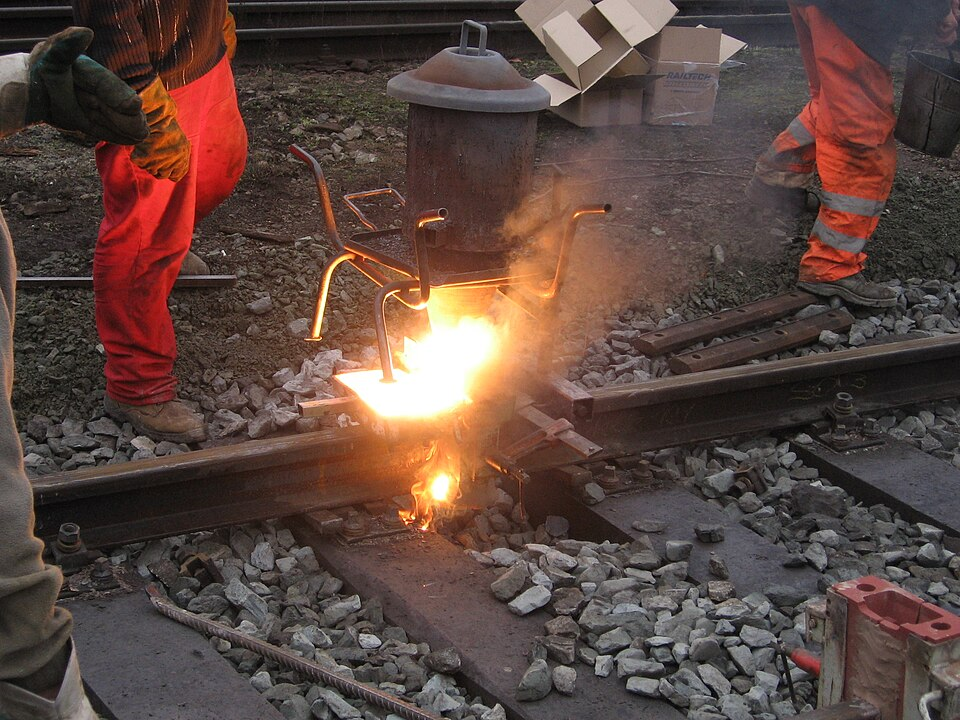
\includegraphics[width=0.5\linewidth]{images/book3/thermite.jpg}

{\small Soudage aluminothermique d'un rail~: la réaction de l'oxyde de fer avec l'aluminium
dans le creuset placé au-dessus du joint donne du fer liquide, qui coule dans le
moule entre les deux extrémités de rail. (Photographie~: PetrS., CC BY-SA 3.0, Wikimedia
Commons.)}
\end{omfigure}

\section{Le carbone et le monoxyde de carbone}

Trois droites font intervenir le carbone~:
\begin{itemize}
  \item \ce{C + O2 -> CO2}~: une mole de gaz en donne une, $\Delta_r S^\circ
        \approx 0$, une droite presque horizontale vers \qty{-395}{kJ}~;
  \item \ce{2C + O2 -> 2CO}~: une mole de gaz en donne deux, $\Delta_r S^\circ
        \approx \qty{+180}{J/(K.mol)}$, une droite qui \emph{descend} avec la température~;
  \item \ce{2CO + O2 -> 2CO2}~: trois moles de gaz en donnent deux, une droite montante.
\end{itemize}

\begin{proposition}[À chaud, le carbone réduit presque tout]\label{prop:b2:ellingham:carbon}
La droite de \ce{2C + O2 -> 2CO} descend avec la température et coupe les
droites de la plupart des oxydes métalliques~: au-dessus de la température de croisement, le carbone réduit
l'oxyde en donnant du monoxyde de carbone. Le croisement avec l'oxyde de fer(II) se situe vers
\qty{1040}{K}, avec l'oxyde de zinc vers \qty{1220}{K}~; pour l'oxyde de titane et la magnésie, il
se situe vers \qty{2000}{K} ou au-delà, pour l'alumine plus haut encore, là où les métaux
se combinent au carbone en carbures ou se réoxydent quand le gaz refroidit.
\end{proposition}

\begin{proof}
La pente $-\Delta_r S^\circ$ de la droite du carbone est négative ($\Delta\nu_{\text{gaz}}
= +1$), celle des droites des oxydes positive~: elles se coupent une fois. Les températures
se lisent sur les droites calculées.
% ledger: janafG:CO.900, janafG:CO.1100, janafG:FeO.900, janafG:FeO.1100 (crossings computed in figdata/bachelor-2/ellingham.py)
\end{proof}

\begin{definition}[Équilibre de Boudouard]\label{def:b2:ellingham:boudouard}
L'\emph{équilibre de Boudouard}\index{equilibre de Boudouard@équilibre de Boudouard} est \ce{C(s) + CO2(g) <=> 2CO(g)},
\omterm{def:b2:reaction-enthalpy:exothermic}{endothermique}, entre le carbone et les deux oxydes de carbone.
\end{definition}

\begin{proposition}[Composition du gaz au contact du carbone]\label{prop:b2:ellingham:boudouard}
Le système carbone + \ce{CO} + \ce{CO2} a pour \omterm{def:b2:equilibrium-shifts:variance}{variance} 2~: à $T$ et pression totale
$p$ données, la fraction molaire $x$ du monoxyde de carbone est fixée par $x^2/(1 - x)
= K^\circ(T)\,p^\circ/p$. Sous \qty{1}{bar}, le gaz est presque uniquement du \ce{CO2}
au-dessous de \qty{700}{K} et presque uniquement du \ce{CO} au-dessus de \qty{1200}{K}~; le croisement des
trois droites du carbone, vers \qty{975}{K}, correspond à $K^\circ = 1$.
\end{proposition}

\begin{proof}
Trois espèces, une réaction, deux phases~: $v = 3 - 1 + 2 - 2 = 2$. Avec $p_{\ce{CO}}
= xp$ et $p_{\ce{CO2}} = (1 - x)p$, $Q = x^2p/[(1 - x)p^\circ]$. Pour $K^\circ = 1$,
les \omterm{def:b2:reaction-free-energy:gibbs-energy}{enthalpies libres} standard de \ce{2C + O2 -> 2CO} et de \ce{C + O2 -> CO2} sont
égales~: les deux droites, et donc la troisième, se coupent.
\end{proof}

\begin{omfigure}
\begin{tikzpicture}
\begin{axis}[
  width=0.62\linewidth, height=5.4cm, xmin=500, xmax=1500, ymin=0, ymax=1.05,
  axis x line=bottom, axis y line=left, xlabel={$T$ (K)},
  xtick={500,700,900,1100,1300,1500}, ytick={0,0.5,1},
  ylabel={fraction molaire de \ce{CO}}, tick label style={font=\small},
  label style={font=\small}, clip=false]
\addplot[omThm, very thick] table[x=T, y=xCO] {figdata/out/bachelor-2-ellingham-b.dat};
\node[font=\scriptsize, anchor=west] at (axis cs:1150,0.55) {\ce{CO} stable};
\node[font=\scriptsize, anchor=west] at (axis cs:510,0.6) {\ce{CO2} (et carbone) stable};
\end{axis}
\end{tikzpicture}

{\small L'\omterm{def:b2:ellingham:boudouard}{équilibre de Boudouard} sous \qty{1}{bar}~: fraction molaire du monoxyde
de carbone dans un gaz en équilibre avec le carbone.}
% ledger: janafG:CO.700, janafG:CO2.700, janafG:CO.1100, janafG:CO2.1100 (computed in figdata/bachelor-2/ellingham.py)
\end{omfigure}

\section{Le haut fourneau}

Le minerai de fer (hématite \ce{Fe2O3}, magnétite \ce{Fe3O4}), le coke et le calcaire sont
chargés au sommet d'une haute cuve~; de l'air chaud est insufflé
près de la base. En descendant, les solides rencontrent un gaz chaud ascendant~; le gaz sort
au sommet, refroidi.
\begin{itemize}
  \item Aux tuyères, le coke brûle dans l'air chaud~: \ce{C + O2 -> CO2} et,
        au-dessus, en présence d'un excès de carbone, \ce{CO2 + C -> 2CO} (Boudouard)~: le gaz
        qui monte est surtout du monoxyde de carbone et du diazote.
  \item Dans la partie haute, le monoxyde de carbone réduit les oxydes de fer étape par
        étape, \ce{3Fe2O3 + CO -> 2Fe3O4 + CO2}, \ce{Fe3O4 + CO -> 3FeO + CO2},
        \ce{FeO + CO -> Fe + CO2}. Les deux premières étapes sont faciles~; pour la dernière,
        la droite \ce{CO}/\ce{CO2} passe un peu \textit{au-dessus} de celle de
        \ce{FeO}~: son \omterm{def:b2:reaction-free-energy:reaction-gibbs}{enthalpie libre standard de réaction} est légèrement positive
        ($K^\circ \approx 0.3$ à \qty{900}{K}), et la réduction exige un gaz
        contenant au moins trois fois plus de \ce{CO} que de \ce{CO2} --- ce que
        l'\omterm{def:b2:ellingham:boudouard}{équilibre de Boudouard} fournit dans la zone chaude située au-dessous.
  \item Plus bas et plus chaud, le carbone lui-même réduit ce qui reste, \ce{FeO + C ->
        Fe + CO}~; le fer dissout du carbone, fond et se rassemble au fond
        sous un laitier fondu formé par la chaux et la silice du minerai.
\end{itemize}

\begin{omfigure}
\begin{tikzpicture}[font=\small, >={Stealth}]
  \fill[gray!12] (-1.4,0) -- (-2.0,3.0) -- (-1.3,7.0) -- (1.3,7.0) -- (2.0,3.0) -- (1.4,0) -- cycle;
  \draw[thick] (-1.4,0) -- (-2.0,3.0) -- (-1.3,7.0) (1.4,0) -- (2.0,3.0) -- (1.3,7.0);
  \draw[thick] (-1.4,0) -- (1.4,0);
  \fill[orange!70!red] (-1.4,0) rectangle (1.4,0.35);
  \fill[yellow!50!orange] (-1.45,0.35) rectangle (1.45,0.6);
  \node[font=\scriptsize] at (0,0.17) {fonte liquide};
  \node[font=\scriptsize] at (0,0.48) {laitier};
  % tuyeres
  \draw[->, thick, omDef] (-3.2,1.2) -- (-1.75,1.2) node[pos=0, left] {air chaud};
  \draw[->, thick, omDef] (3.2,1.2) -- (1.75,1.2);
  % charge and gas
  \draw[->, thick] (-0.6,7.9) -- (-0.6,7.1) node[pos=0, above left, xshift=6pt] {minerai, coke, calcaire};
  \draw[->, thick, omThm] (0.7,7.1) -- (0.7,7.9) node[pos=1, above right, xshift=-6pt] {gaz de gueulard (\ce{CO}, \ce{CO2}, \ce{N2})};
  \draw[->, omThm, thick] (0.6,1.6) -- (0.6,6.4);
  \draw[->, thick] (-0.6,6.4) -- (-0.6,1.6);
  \node[omThm, font=\scriptsize, rotate=90] at (0.9,4.0) {le gaz monte};
  \node[font=\scriptsize, rotate=90] at (-0.9,4.0) {les solides descendent};
  % zones
  \node[anchor=west, align=left, font=\scriptsize] at (2.3,6.0) {\ce{3Fe2O3 + CO -> 2Fe3O4 + CO2}\\ \ce{Fe3O4 + CO -> 3FeO + CO2}};
  \node[anchor=west, align=left, font=\scriptsize] at (2.3,4.2) {\ce{FeO + CO -> Fe + CO2}};
  \node[anchor=west, align=left, font=\scriptsize] at (2.3,2.7) {\ce{CO2 + C -> 2CO}\\ \ce{FeO + C -> Fe + CO}};
  \node[anchor=west, align=left, font=\scriptsize] at (2.3,1.6) {\ce{C + O2 -> CO2}};
  \draw[densely dotted] (1.95,6.0) -- (2.3,6.0) (1.9,4.2) -- (2.3,4.2) (2.0,2.8) -- (2.3,2.8);
  \node[anchor=east, align=right, font=\scriptsize, black!60] at (-2.2,6.0) {plus froid};
  \node[anchor=east, align=right, font=\scriptsize, black!60] at (-2.2,2.3) {plus chaud};
  \draw[->, black!50] (-2.6,5.6) -- (-2.6,2.7);
\end{tikzpicture}

{\small Le haut fourneau, réacteur à contre-courant. Les solides descendent, le gaz
réducteur chaud monte~; les oxydes de fer sont réduits par le monoxyde de carbone dans la
partie haute, plus froide, et par le carbone dans la partie basse, plus chaude. La fonte et le laitier
sont coulés à la base.}
\end{omfigure}

\begin{omfigure}
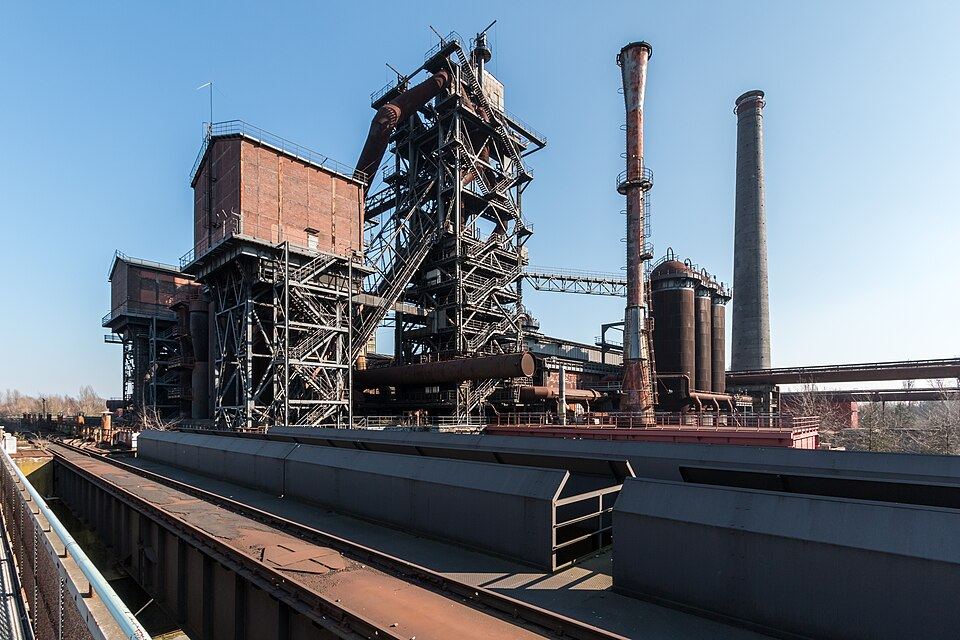
\includegraphics[width=0.6\linewidth]{images/book3/blast-furnace.jpg}

{\small Un haut fourneau conservé comme monument (Duisburg-Nord, arrêté en
1985)~: la haute cuve avec sa couronne de conduites d'air chaud, les prises de gaz
au sommet. (Photographie~: Dietmar Rabich, CC BY-SA 4.0, Wikimedia Commons.)}
\end{omfigure}

\section{Autres voies d'obtention d'un métal}

\begin{definition}[Pyrométallurgie et hydrométallurgie]\label{def:b2:ellingham:metallurgy}
La \emph{pyrométallurgie}\index{pyrometallurgie@pyrométallurgie} extrait un métal à haute
température, par réduction de son oxyde dans un four. L'\emph{hydrométallurgie}\index{hydrometallurgie@hydrométallurgie}
l'extrait d'une solution aqueuse. Leurs étapes usuelles sont le
\emph{grillage}\index{grillage} (chauffage d'un minerai sulfuré dans l'air pour le transformer en
oxyde, \ce{2ZnS + 3O2 -> 2ZnO + 2SO2}), la \emph{lixiviation}\index{lixiviation}
(mise en solution du composé du métal, souvent dans l'acide sulfurique, \ce{ZnO + 2H+ ->
Zn^2+ + H2O}), la purification de la solution, par exemple par
\emph{cémentation}\index{cementation@cémentation} (réduction des ions d'un métal plus noble
par la poudre d'un métal moins noble, \ce{Cu^2+ + Zn -> Cu + Zn^2+}), et la
récupération du métal, souvent par électrolyse.
\end{definition}

Le diagramme explique ce partage des tâches. Le fer, le zinc, le plomb, l'étain sont obtenus par
le carbone dans un four. L'aluminium, dont la droite est bien au-dessous de celle du carbone à toute
température praticable, est produit par électrolyse de son oxyde fondu
(\cref{ch:b2:batteries-electrolysis})~; le magnésium par électrolyse ou par
réduction par le silicium sous vide, qui élimine la vapeur de magnésium~;
le titane en transformant l'oxyde en chlorure, \ce{TiO2 + 2Cl2 + C -> TiCl4 +
CO2} (\cref{exo:b2:reaction-free-energy:12}), puis en réduisant le chlorure par
le magnésium (procédé Kroll). La majeure partie du zinc mondial est produite par \omterm{def:b2:ellingham:metallurgy}{grillage},
\omterm{def:b2:ellingham:metallurgy}{lixiviation} et électrolyse~: la voie hydrométallurgique donne un métal plus pur et
évite de manipuler de la vapeur de zinc.

\begin{omfigure}
\begin{tikzpicture}[font=\small, >={Stealth}, box/.style={draw, thick, rounded corners=2pt, align=center, minimum height=0.9cm, fill=white, text width=2.3cm}]
  \node[box] (r) at (0,0) {grillage\\ \ce{ZnS} $\to$ \ce{ZnO}};
  \node[box] (l) at (3.2,0) {lixiviation\\ dans \ce{H2SO4}};
  \node[box] (c) at (6.4,0) {purification\\ (cémentation)};
  \node[box] (e) at (9.6,0) {électrolyse\\ \ce{Zn^2+} $\to$ \ce{Zn}};
  \draw[->, thick] (r) -- (l); \draw[->, thick] (l) -- (c); \draw[->, thick] (c) -- (e);
  \draw[->, thick, black!60] (r.north) -- ++(0,0.7) node[above] {\ce{SO2} $\to$ acide sulfurique};
  \draw[->, thick, omThm] (e.south) -- ++(0,-0.6) -| (l.south) node[pos=0.25, below] {acide recyclé};
  \draw[->, thick] (e.east) -- ++(0.8,0) node[right] {zinc};
\end{tikzpicture}

{\small La voie hydrométallurgique du zinc. Le dioxyde de soufre du four de \omterm{def:b2:ellingham:metallurgy}{grillage}
est transformé en l'acide sulfurique de la \omterm{def:b2:ellingham:metallurgy}{lixiviation}~; l'acide régénéré à
l'anode de l'électrolyse y est renvoyé.}
\end{omfigure}

\section{Exercices}

\begin{exercise}[$\star$]\label{exo:b2:ellingham:1}
Écrire les réactions représentées par les droites de l'oxyde de cuivre(I), de l'alumine, du monoxyde
de carbone et du dioxyde de carbone, chacune pour une mole de \ce{O2}.
\end{exercise}

\begin{exercise}[$\star$]\label{exo:b2:ellingham:2}
À partir des valeurs clés du CODATA ($\Delta_f H^\circ(\ce{ZnO}) = \qty{-350.46}{kJ/mol}$,
$S^\circ$~: \ce{ZnO} 43.65, \ce{Zn} 41.63, \ce{O2} \qty{205.15}{J/(K.mol)}),
écrire le $\Delta_r G^\circ(T)$ de \ce{2Zn + O2 -> 2ZnO} pour le zinc solide.
\end{exercise}

\begin{exercise}[$\star$]\label{exo:b2:ellingham:3}
À l'aide du diagramme, dresser la liste des métaux qui peuvent réduire l'oxyde de chrome(III) à
\qty{1500}{K}, et de ceux qui ne le peuvent pas.
\end{exercise}

\begin{exercise}[$\star$]\label{exo:b2:ellingham:4}
Expliquer le signe de la pente de chacune des trois droites du carbone.
\end{exercise}

\begin{exercise}[$\star\star$]\label{exo:b2:ellingham:5}
Calculer la \omterm{def:b2:ellingham:oxygen-pressure}{pression de dioxygène à l'équilibre} de l'oxyde de mercure(II) à \qty{600}{K}
(mercure liquide, $\Delta_r H^\circ = \qty{-181.6}{kJ}$, $\Delta_r S^\circ =
\qty{-216.5}{J/K}$ par mole de \ce{O2}). Le mercure est-il oxydé dans l'air à cette
température~?
\end{exercise}

\begin{exercise}[$\star\star$]\label{exo:b2:ellingham:6}
Calculer le $\Delta_r G^\circ$ à \qty{298}{K} de la réaction de la thermite, \ce{Fe2O3 +
2Al -> Al2O3 + 2Fe}, sachant que $\Delta_f G^\circ = \qty{-743.5}{kJ/mol}$ pour
\ce{Fe2O3} et \qty{-1582.3}{kJ/mol} pour \ce{Al2O3}, et dire pourquoi la réaction,
bien que très \omterm{def:b2:reaction-free-energy:exergonic}{exergonique}, ne démarre pas à température ambiante.
% ledger: janafG:Fe2O3.298, janafG:Al2O3.298
\end{exercise}

\begin{exercise}[$\star\star$]\label{exo:b2:ellingham:7}
Trouver sur le diagramme la température au-dessus de laquelle le carbone réduit l'oxyde de fer(II)
en fer avec formation de monoxyde de carbone, et écrire la réaction.
\end{exercise}

\begin{exercise}[$\star\star$]\label{exo:b2:ellingham:8}
À \qty{1100}{K}, $\Delta_f G^\circ(\ce{CO}) = \qty{-209.1}{kJ/mol}$ et
$\Delta_f G^\circ(\ce{CO2}) = \qty{-396.0}{kJ/mol}$. Calculer le $K^\circ$ de
l'\omterm{def:b2:ellingham:boudouard}{équilibre de Boudouard} et la fraction molaire du monoxyde de carbone au contact du carbone sous
\qty{1}{bar}. Qu'advient-il du gaz, au contact de suie ou de fer, lorsqu'on le
refroidit à \qty{700}{K}~?
% ledger: janafG:CO.1100, janafG:CO2.1100
\end{exercise}

\begin{exercise}[$\star\star$]\label{exo:b2:ellingham:9}
On utilise parfois le dihydrogène pour réduire l'oxyde de tungstène. À l'aide de la droite de l'eau,
expliquer pourquoi le dihydrogène est un meilleur réducteur que le monoxyde de carbone à haute
température mais un moins bon à basse température.
\end{exercise}

\begin{exercise}[$\star\star\star$]\label{exo:b2:ellingham:10}
L'oxyde de magnésium peut être réduit par le silicium, \ce{2MgO + Si -> SiO2 + 2Mg}, bien que
la droite de la silice soit au-dessus de celle de la magnésie à toute température du
diagramme. À \qty{1500}{K}, le magnésium est gazeux et les tables donnent, par mole de
\ce{O2}, \qty{-845.5}{kJ} pour la magnésie et \qty{-643.7}{kJ} pour la silice.
Calculer le $\Delta_r G^\circ$ de la réduction, puis la pression de vapeur de magnésium
au-dessous de laquelle elle se produit dans le sens direct. Comment un four sous vide en tire-t-il parti~?
% ledger: janafG:MgO.1500, janafG:SiO2.1500
\end{exercise}

\begin{exercise}[$\star\star\star$]\label{exo:b2:ellingham:11}
Calculer la \omterm{def:b2:equilibrium-shifts:variance}{variance} du système \ce{FeO(s)}, \ce{Fe(s)}, \ce{CO(g)},
\ce{CO2(g)} à l'équilibre. Qu'est-ce que cela signifie pour le gaz qui quitte la partie haute
d'un haut fourneau~?
\end{exercise}

\begin{exercise}[$\star\star\star$]\label{exo:b2:ellingham:12}
Le cuivre est purifié de sa solution de \omterm{def:b2:ellingham:metallurgy}{lixiviation} par \omterm{def:b2:ellingham:metallurgy}{cémentation} avec des déchets de fer.
À l'aide des potentiels standard du volume de première année ($E^\circ(\ce{Cu^2+}/\ce{Cu})
= \qty{0.34}{V}$, $E^\circ(\ce{Fe^2+}/\ce{Fe}) = \qty{-0.41}{V}$), calculer la
constante d'équilibre de \ce{Cu^2+ + Fe -> Cu + Fe^2+} et la concentration résiduelle
en ions cuivre lorsque la solution contient \qty{1.0}{mol/L} de
\ce{Fe^2+}.
\end{exercise}

\section{Problème~: le zinc par le feu}

\begin{problem}[{Problème du week-end --- les droites d'Ellingham de l'oxyde de zinc et du
monoxyde de carbone, la température à laquelle le carbone réduit l'oxyde de zinc, la
variance du four, et la condensation de la vapeur de zinc}]
\label{pb:b2:ellingham:1}
Avant l'électrolyse, on produisait le zinc en chauffant son oxyde avec du carbone dans des cornues
en argile. Données (CODATA, et table JANAF du zinc)~: $\Delta_f H^\circ(\ce{ZnO})
= \qty{-350.46}{kJ/mol}$~; $S^\circ$ (\unit{J/(K.mol)})~: \ce{ZnO} 43.65, \ce{Zn}
41.63, \ce{O2} 205.15~; le zinc fond à \qty{692.7}{K} ($\Delta_{\text{fus}}H =
\qty{7.32}{kJ/mol}$) et bout à \qty{1180.2}{K} sous \qty{1}{bar}
($\Delta_{\text{vap}}H = \qty{115.3}{kJ/mol}$). Pour \ce{2C + O2 -> 2CO}, les
tables donnent $\Delta_r G^\circ = \qty{-418.2}{kJ}$ à \qty{1100}{K} et
\qty{-453.0}{kJ} à \qty{1300}{K}.
% ledger: dfh:ZnO_cr, s0:ZnO_cr, s0:Zn_cr, s0:O2_g, hT:Zn_cr.692, hT:Zn_l.692, hT:Zn_l.1180, hT:Zn_g.1180, dfh:Zn_g, janafG:CO.1100, janafG:CO.1300

\medskip
\noindent\textbf{Partie I --- La droite de l'oxyde de zinc.}
\begin{enumerate}
  \item Calculer $\Delta_r H^\circ$ et $\Delta_r S^\circ$ de \ce{2Zn(s) + O2 ->
        2ZnO} à \qty{298}{K}.
  \item Écrire $\Delta_r G^\circ(T)$ au-dessous de la température de fusion.
  \item Calculer les entropies de fusion et de vaporisation du zinc.
  \item Écrire $\Delta_r G^\circ(T)$ entre les températures de fusion et d'ébullition.
  \item L'écrire au-dessus de la température d'ébullition.
  \item Calculer les trois pentes et expliquer pourquoi la dernière est bien plus forte.
  \item Vérifier que les trois expressions concordent aux températures de changement d'état.
\end{enumerate}

\medskip
\noindent\textbf{Partie II --- La droite du carbone.}
\begin{enumerate}[resume]
  \item À partir des deux valeurs tabulées, écrire la droite de \ce{2C + O2 -> 2CO} sous
        la forme $a + bT$ entre \qty{1100}{K} et \qty{1300}{K}.
  \item En déduire son $\Delta_r S^\circ$ et expliquer son signe.
  \item Écrire la réduction \ce{ZnO + C -> Zn(g) + CO} et son $\Delta_r
        G^\circ(T)$ comme différence des deux droites (par mole de \ce{O2}).
  \item Trouver la température où les deux droites se coupent.
  \item Pourquoi est-il important que cette température soit supérieure à la température d'ébullition
        du zinc~?
\end{enumerate}

\medskip
\noindent\textbf{Partie III --- La cornue.}
\begin{enumerate}[resume]
  \item Calculer la \omterm{def:b2:equilibrium-shifts:variance}{variance} du système \ce{ZnO(s)}, \ce{C(s)}, \ce{Zn(g)},
        \ce{CO(g)}, le zinc et le monoxyde de carbone n'étant formés que par la réduction.
  \item Dans une cornue à \qty{1300}{K} sous \qty{1}{bar}, quelles sont les pressions
        partielles du zinc et du monoxyde de carbone si la réaction est totale~?
  \item Calculer le $\Delta_r G^\circ$ de la réduction à \qty{1300}{K} et le
        $K^\circ$ correspondant.
  \item Expliquer pourquoi on fait fonctionner la cornue un peu au-dessus de la température de
        croisement et non très au-dessus.
\end{enumerate}

\medskip
\noindent\textbf{Partie IV --- Le condenseur.}
\begin{enumerate}[resume]
  \item La vapeur est conduite dans un condenseur plus froid. Écrire la réaction par laquelle
        la vapeur de zinc peut être réoxydée par le dioxyde de carbone.
  \item À l'aide du diagramme, expliquer pourquoi le gaz doit être exempt de dioxyde
        de carbone.
  \item Pourquoi faut-il condenser le zinc rapidement plutôt que lentement~?
  \item Calculer la masse de carbone nécessaire par tonne de zinc, la
        réduction étant prise telle qu'elle est écrite.
  \item Calculer la chaleur absorbée par tonne de zinc par la réduction vers
        \qty{1300}{K} (prendre $\Delta_r H^\circ$ dans les expressions des parties I
        et II).
  \item Donner la température au-dessus de laquelle le carbone réduit l'oxyde de zinc dans
        les conditions standard.
\end{enumerate}
\end{problem}
